\documentclass[10pt]{article}
\usepackage{tmlr}
% Camera-ready: \usepackage[accepted]{tmlr}   Preprint: \usepackage[preprint]{tmlr}

%%%%% NEW MATH DEFINITIONS %%%%%

\usepackage{amsmath,amsfonts,bm}

% Mark sections of captions for referring to divisions of figures
\newcommand{\figleft}{{\em (Left)}}
\newcommand{\figcenter}{{\em (Center)}}
\newcommand{\figright}{{\em (Right)}}
\newcommand{\figtop}{{\em (Top)}}
\newcommand{\figbottom}{{\em (Bottom)}}
\newcommand{\captiona}{{\em (a)}}
\newcommand{\captionb}{{\em (b)}}
\newcommand{\captionc}{{\em (c)}}
\newcommand{\captiond}{{\em (d)}}

% Highlight a newly defined term
\newcommand{\newterm}[1]{{\bf #1}}


% Figure reference, lower-case.
\def\figref#1{figure~\ref{#1}}
% Figure reference, capital. For start of sentence
\def\Figref#1{Figure~\ref{#1}}
\def\twofigref#1#2{figures \ref{#1} and \ref{#2}}
\def\quadfigref#1#2#3#4{figures \ref{#1}, \ref{#2}, \ref{#3} and \ref{#4}}
% Section reference, lower-case.
\def\secref#1{section~\ref{#1}}
% Section reference, capital.
\def\Secref#1{Section~\ref{#1}}
% Reference to two sections.
\def\twosecrefs#1#2{sections \ref{#1} and \ref{#2}}
% Reference to three sections.
\def\secrefs#1#2#3{sections \ref{#1}, \ref{#2} and \ref{#3}}
% Reference to an equation, lower-case.
\def\eqref#1{equation~\ref{#1}}
% Reference to an equation, upper case
\def\Eqref#1{Equation~\ref{#1}}
% A raw reference to an equation---avoid using if possible
\def\plaineqref#1{\ref{#1}}
% Reference to a chapter, lower-case.
\def\chapref#1{chapter~\ref{#1}}
% Reference to an equation, upper case.
\def\Chapref#1{Chapter~\ref{#1}}
% Reference to a range of chapters
\def\rangechapref#1#2{chapters\ref{#1}--\ref{#2}}
% Reference to an algorithm, lower-case.
\def\algref#1{algorithm~\ref{#1}}
% Reference to an algorithm, upper case.
\def\Algref#1{Algorithm~\ref{#1}}
\def\twoalgref#1#2{algorithms \ref{#1} and \ref{#2}}
\def\Twoalgref#1#2{Algorithms \ref{#1} and \ref{#2}}
% Reference to a part, lower case
\def\partref#1{part~\ref{#1}}
% Reference to a part, upper case
\def\Partref#1{Part~\ref{#1}}
\def\twopartref#1#2{parts \ref{#1} and \ref{#2}}

\def\ceil#1{\lceil #1 \rceil}
\def\floor#1{\lfloor #1 \rfloor}
\def\1{\bm{1}}
\newcommand{\train}{\mathcal{D}}
\newcommand{\valid}{\mathcal{D_{\mathrm{valid}}}}
\newcommand{\test}{\mathcal{D_{\mathrm{test}}}}

\def\eps{{\epsilon}}


% Random variables
\def\reta{{\textnormal{$\eta$}}}
\def\ra{{\textnormal{a}}}
\def\rb{{\textnormal{b}}}
\def\rc{{\textnormal{c}}}
\def\rd{{\textnormal{d}}}
\def\re{{\textnormal{e}}}
\def\rf{{\textnormal{f}}}
\def\rg{{\textnormal{g}}}
\def\rh{{\textnormal{h}}}
\def\ri{{\textnormal{i}}}
\def\rj{{\textnormal{j}}}
\def\rk{{\textnormal{k}}}
\def\rl{{\textnormal{l}}}
% rm is already a command, just don't name any random variables m
\def\rn{{\textnormal{n}}}
\def\ro{{\textnormal{o}}}
\def\rp{{\textnormal{p}}}
\def\rq{{\textnormal{q}}}
\def\rr{{\textnormal{r}}}
\def\rs{{\textnormal{s}}}
\def\rt{{\textnormal{t}}}
\def\ru{{\textnormal{u}}}
\def\rv{{\textnormal{v}}}
\def\rw{{\textnormal{w}}}
\def\rx{{\textnormal{x}}}
\def\ry{{\textnormal{y}}}
\def\rz{{\textnormal{z}}}

% Random vectors
\def\rvepsilon{{\mathbf{\epsilon}}}
\def\rvtheta{{\mathbf{\theta}}}
\def\rva{{\mathbf{a}}}
\def\rvb{{\mathbf{b}}}
\def\rvc{{\mathbf{c}}}
\def\rvd{{\mathbf{d}}}
\def\rve{{\mathbf{e}}}
\def\rvf{{\mathbf{f}}}
\def\rvg{{\mathbf{g}}}
\def\rvh{{\mathbf{h}}}
\def\rvu{{\mathbf{i}}}
\def\rvj{{\mathbf{j}}}
\def\rvk{{\mathbf{k}}}
\def\rvl{{\mathbf{l}}}
\def\rvm{{\mathbf{m}}}
\def\rvn{{\mathbf{n}}}
\def\rvo{{\mathbf{o}}}
\def\rvp{{\mathbf{p}}}
\def\rvq{{\mathbf{q}}}
\def\rvr{{\mathbf{r}}}
\def\rvs{{\mathbf{s}}}
\def\rvt{{\mathbf{t}}}
\def\rvu{{\mathbf{u}}}
\def\rvv{{\mathbf{v}}}
\def\rvw{{\mathbf{w}}}
\def\rvx{{\mathbf{x}}}
\def\rvy{{\mathbf{y}}}
\def\rvz{{\mathbf{z}}}

% Elements of random vectors
\def\erva{{\textnormal{a}}}
\def\ervb{{\textnormal{b}}}
\def\ervc{{\textnormal{c}}}
\def\ervd{{\textnormal{d}}}
\def\erve{{\textnormal{e}}}
\def\ervf{{\textnormal{f}}}
\def\ervg{{\textnormal{g}}}
\def\ervh{{\textnormal{h}}}
\def\ervi{{\textnormal{i}}}
\def\ervj{{\textnormal{j}}}
\def\ervk{{\textnormal{k}}}
\def\ervl{{\textnormal{l}}}
\def\ervm{{\textnormal{m}}}
\def\ervn{{\textnormal{n}}}
\def\ervo{{\textnormal{o}}}
\def\ervp{{\textnormal{p}}}
\def\ervq{{\textnormal{q}}}
\def\ervr{{\textnormal{r}}}
\def\ervs{{\textnormal{s}}}
\def\ervt{{\textnormal{t}}}
\def\ervu{{\textnormal{u}}}
\def\ervv{{\textnormal{v}}}
\def\ervw{{\textnormal{w}}}
\def\ervx{{\textnormal{x}}}
\def\ervy{{\textnormal{y}}}
\def\ervz{{\textnormal{z}}}

% Random matrices
\def\rmA{{\mathbf{A}}}
\def\rmB{{\mathbf{B}}}
\def\rmC{{\mathbf{C}}}
\def\rmD{{\mathbf{D}}}
\def\rmE{{\mathbf{E}}}
\def\rmF{{\mathbf{F}}}
\def\rmG{{\mathbf{G}}}
\def\rmH{{\mathbf{H}}}
\def\rmI{{\mathbf{I}}}
\def\rmJ{{\mathbf{J}}}
\def\rmK{{\mathbf{K}}}
\def\rmL{{\mathbf{L}}}
\def\rmM{{\mathbf{M}}}
\def\rmN{{\mathbf{N}}}
\def\rmO{{\mathbf{O}}}
\def\rmP{{\mathbf{P}}}
\def\rmQ{{\mathbf{Q}}}
\def\rmR{{\mathbf{R}}}
\def\rmS{{\mathbf{S}}}
\def\rmT{{\mathbf{T}}}
\def\rmU{{\mathbf{U}}}
\def\rmV{{\mathbf{V}}}
\def\rmW{{\mathbf{W}}}
\def\rmX{{\mathbf{X}}}
\def\rmY{{\mathbf{Y}}}
\def\rmZ{{\mathbf{Z}}}

% Elements of random matrices
\def\ermA{{\textnormal{A}}}
\def\ermB{{\textnormal{B}}}
\def\ermC{{\textnormal{C}}}
\def\ermD{{\textnormal{D}}}
\def\ermE{{\textnormal{E}}}
\def\ermF{{\textnormal{F}}}
\def\ermG{{\textnormal{G}}}
\def\ermH{{\textnormal{H}}}
\def\ermI{{\textnormal{I}}}
\def\ermJ{{\textnormal{J}}}
\def\ermK{{\textnormal{K}}}
\def\ermL{{\textnormal{L}}}
\def\ermM{{\textnormal{M}}}
\def\ermN{{\textnormal{N}}}
\def\ermO{{\textnormal{O}}}
\def\ermP{{\textnormal{P}}}
\def\ermQ{{\textnormal{Q}}}
\def\ermR{{\textnormal{R}}}
\def\ermS{{\textnormal{S}}}
\def\ermT{{\textnormal{T}}}
\def\ermU{{\textnormal{U}}}
\def\ermV{{\textnormal{V}}}
\def\ermW{{\textnormal{W}}}
\def\ermX{{\textnormal{X}}}
\def\ermY{{\textnormal{Y}}}
\def\ermZ{{\textnormal{Z}}}

% Vectors
\def\vzero{{\bm{0}}}
\def\vone{{\bm{1}}}
\def\vmu{{\bm{\mu}}}
\def\vtheta{{\bm{\theta}}}
\def\va{{\bm{a}}}
\def\vb{{\bm{b}}}
\def\vc{{\bm{c}}}
\def\vd{{\bm{d}}}
\def\ve{{\bm{e}}}
\def\vf{{\bm{f}}}
\def\vg{{\bm{g}}}
\def\vh{{\bm{h}}}
\def\vi{{\bm{i}}}
\def\vj{{\bm{j}}}
\def\vk{{\bm{k}}}
\def\vl{{\bm{l}}}
\def\vm{{\bm{m}}}
\def\vn{{\bm{n}}}
\def\vo{{\bm{o}}}
\def\vp{{\bm{p}}}
\def\vq{{\bm{q}}}
\def\vr{{\bm{r}}}
\def\vs{{\bm{s}}}
\def\vt{{\bm{t}}}
\def\vu{{\bm{u}}}
\def\vv{{\bm{v}}}
\def\vw{{\bm{w}}}
\def\vx{{\bm{x}}}
\def\vy{{\bm{y}}}
\def\vz{{\bm{z}}}

% Elements of vectors
\def\evalpha{{\alpha}}
\def\evbeta{{\beta}}
\def\evepsilon{{\epsilon}}
\def\evlambda{{\lambda}}
\def\evomega{{\omega}}
\def\evmu{{\mu}}
\def\evpsi{{\psi}}
\def\evsigma{{\sigma}}
\def\evtheta{{\theta}}
\def\eva{{a}}
\def\evb{{b}}
\def\evc{{c}}
\def\evd{{d}}
\def\eve{{e}}
\def\evf{{f}}
\def\evg{{g}}
\def\evh{{h}}
\def\evi{{i}}
\def\evj{{j}}
\def\evk{{k}}
\def\evl{{l}}
\def\evm{{m}}
\def\evn{{n}}
\def\evo{{o}}
\def\evp{{p}}
\def\evq{{q}}
\def\evr{{r}}
\def\evs{{s}}
\def\evt{{t}}
\def\evu{{u}}
\def\evv{{v}}
\def\evw{{w}}
\def\evx{{x}}
\def\evy{{y}}
\def\evz{{z}}

% Matrix
\def\mA{{\bm{A}}}
\def\mB{{\bm{B}}}
\def\mC{{\bm{C}}}
\def\mD{{\bm{D}}}
\def\mE{{\bm{E}}}
\def\mF{{\bm{F}}}
\def\mG{{\bm{G}}}
\def\mH{{\bm{H}}}
\def\mI{{\bm{I}}}
\def\mJ{{\bm{J}}}
\def\mK{{\bm{K}}}
\def\mL{{\bm{L}}}
\def\mM{{\bm{M}}}
\def\mN{{\bm{N}}}
\def\mO{{\bm{O}}}
\def\mP{{\bm{P}}}
\def\mQ{{\bm{Q}}}
\def\mR{{\bm{R}}}
\def\mS{{\bm{S}}}
\def\mT{{\bm{T}}}
\def\mU{{\bm{U}}}
\def\mV{{\bm{V}}}
\def\mW{{\bm{W}}}
\def\mX{{\bm{X}}}
\def\mY{{\bm{Y}}}
\def\mZ{{\bm{Z}}}
\def\mBeta{{\bm{\beta}}}
\def\mPhi{{\bm{\Phi}}}
\def\mLambda{{\bm{\Lambda}}}
\def\mSigma{{\bm{\Sigma}}}

% Tensor
\DeclareMathAlphabet{\mathsfit}{\encodingdefault}{\sfdefault}{m}{sl}
\SetMathAlphabet{\mathsfit}{bold}{\encodingdefault}{\sfdefault}{bx}{n}
\newcommand{\tens}[1]{\bm{\mathsfit{#1}}}
\def\tA{{\tens{A}}}
\def\tB{{\tens{B}}}
\def\tC{{\tens{C}}}
\def\tD{{\tens{D}}}
\def\tE{{\tens{E}}}
\def\tF{{\tens{F}}}
\def\tG{{\tens{G}}}
\def\tH{{\tens{H}}}
\def\tI{{\tens{I}}}
\def\tJ{{\tens{J}}}
\def\tK{{\tens{K}}}
\def\tL{{\tens{L}}}
\def\tM{{\tens{M}}}
\def\tN{{\tens{N}}}
\def\tO{{\tens{O}}}
\def\tP{{\tens{P}}}
\def\tQ{{\tens{Q}}}
\def\tR{{\tens{R}}}
\def\tS{{\tens{S}}}
\def\tT{{\tens{T}}}
\def\tU{{\tens{U}}}
\def\tV{{\tens{V}}}
\def\tW{{\tens{W}}}
\def\tX{{\tens{X}}}
\def\tY{{\tens{Y}}}
\def\tZ{{\tens{Z}}}


% Graph
\def\gA{{\mathcal{A}}}
\def\gB{{\mathcal{B}}}
\def\gC{{\mathcal{C}}}
\def\gD{{\mathcal{D}}}
\def\gE{{\mathcal{E}}}
\def\gF{{\mathcal{F}}}
\def\gG{{\mathcal{G}}}
\def\gH{{\mathcal{H}}}
\def\gI{{\mathcal{I}}}
\def\gJ{{\mathcal{J}}}
\def\gK{{\mathcal{K}}}
\def\gL{{\mathcal{L}}}
\def\gM{{\mathcal{M}}}
\def\gN{{\mathcal{N}}}
\def\gO{{\mathcal{O}}}
\def\gP{{\mathcal{P}}}
\def\gQ{{\mathcal{Q}}}
\def\gR{{\mathcal{R}}}
\def\gS{{\mathcal{S}}}
\def\gT{{\mathcal{T}}}
\def\gU{{\mathcal{U}}}
\def\gV{{\mathcal{V}}}
\def\gW{{\mathcal{W}}}
\def\gX{{\mathcal{X}}}
\def\gY{{\mathcal{Y}}}
\def\gZ{{\mathcal{Z}}}

% Sets
\def\sA{{\mathbb{A}}}
\def\sB{{\mathbb{B}}}
\def\sC{{\mathbb{C}}}
\def\sD{{\mathbb{D}}}
% Don't use a set called E, because this would be the same as our symbol
% for expectation.
\def\sF{{\mathbb{F}}}
\def\sG{{\mathbb{G}}}
\def\sH{{\mathbb{H}}}
\def\sI{{\mathbb{I}}}
\def\sJ{{\mathbb{J}}}
\def\sK{{\mathbb{K}}}
\def\sL{{\mathbb{L}}}
\def\sM{{\mathbb{M}}}
\def\sN{{\mathbb{N}}}
\def\sO{{\mathbb{O}}}
\def\sP{{\mathbb{P}}}
\def\sQ{{\mathbb{Q}}}
\def\sR{{\mathbb{R}}}
\def\sS{{\mathbb{S}}}
\def\sT{{\mathbb{T}}}
\def\sU{{\mathbb{U}}}
\def\sV{{\mathbb{V}}}
\def\sW{{\mathbb{W}}}
\def\sX{{\mathbb{X}}}
\def\sY{{\mathbb{Y}}}
\def\sZ{{\mathbb{Z}}}

% Entries of a matrix
\def\emLambda{{\Lambda}}
\def\emA{{A}}
\def\emB{{B}}
\def\emC{{C}}
\def\emD{{D}}
\def\emE{{E}}
\def\emF{{F}}
\def\emG{{G}}
\def\emH{{H}}
\def\emI{{I}}
\def\emJ{{J}}
\def\emK{{K}}
\def\emL{{L}}
\def\emM{{M}}
\def\emN{{N}}
\def\emO{{O}}
\def\emP{{P}}
\def\emQ{{Q}}
\def\emR{{R}}
\def\emS{{S}}
\def\emT{{T}}
\def\emU{{U}}
\def\emV{{V}}
\def\emW{{W}}
\def\emX{{X}}
\def\emY{{Y}}
\def\emZ{{Z}}
\def\emSigma{{\Sigma}}

% entries of a tensor
% Same font as tensor, without \bm wrapper
\newcommand{\etens}[1]{\mathsfit{#1}}
\def\etLambda{{\etens{\Lambda}}}
\def\etA{{\etens{A}}}
\def\etB{{\etens{B}}}
\def\etC{{\etens{C}}}
\def\etD{{\etens{D}}}
\def\etE{{\etens{E}}}
\def\etF{{\etens{F}}}
\def\etG{{\etens{G}}}
\def\etH{{\etens{H}}}
\def\etI{{\etens{I}}}
\def\etJ{{\etens{J}}}
\def\etK{{\etens{K}}}
\def\etL{{\etens{L}}}
\def\etM{{\etens{M}}}
\def\etN{{\etens{N}}}
\def\etO{{\etens{O}}}
\def\etP{{\etens{P}}}
\def\etQ{{\etens{Q}}}
\def\etR{{\etens{R}}}
\def\etS{{\etens{S}}}
\def\etT{{\etens{T}}}
\def\etU{{\etens{U}}}
\def\etV{{\etens{V}}}
\def\etW{{\etens{W}}}
\def\etX{{\etens{X}}}
\def\etY{{\etens{Y}}}
\def\etZ{{\etens{Z}}}

% The true underlying data generating distribution
\newcommand{\pdata}{p_{\rm{data}}}
% The empirical distribution defined by the training set
\newcommand{\ptrain}{\hat{p}_{\rm{data}}}
\newcommand{\Ptrain}{\hat{P}_{\rm{data}}}
% The model distribution
\newcommand{\pmodel}{p_{\rm{model}}}
\newcommand{\Pmodel}{P_{\rm{model}}}
\newcommand{\ptildemodel}{\tilde{p}_{\rm{model}}}
% Stochastic autoencoder distributions
\newcommand{\pencode}{p_{\rm{encoder}}}
\newcommand{\pdecode}{p_{\rm{decoder}}}
\newcommand{\precons}{p_{\rm{reconstruct}}}

\newcommand{\laplace}{\mathrm{Laplace}} % Laplace distribution

\newcommand{\E}{\mathbb{E}}
\newcommand{\Ls}{\mathcal{L}}
\newcommand{\R}{\mathbb{R}}
\newcommand{\emp}{\tilde{p}}
\newcommand{\lr}{\alpha}
\newcommand{\reg}{\lambda}
\newcommand{\rect}{\mathrm{rectifier}}
\newcommand{\softmax}{\mathrm{softmax}}
\newcommand{\sigmoid}{\sigma}
\newcommand{\softplus}{\zeta}
\newcommand{\KL}{D_{\mathrm{KL}}}
\newcommand{\Var}{\mathrm{Var}}
\newcommand{\standarderror}{\mathrm{SE}}
\newcommand{\Cov}{\mathrm{Cov}}
% Wolfram Mathworld says $L^2$ is for function spaces and $\ell^2$ is for vectors
% But then they seem to use $L^2$ for vectors throughout the site, and so does
% wikipedia.
\newcommand{\normlzero}{L^0}
\newcommand{\normlone}{L^1}
\newcommand{\normltwo}{L^2}
\newcommand{\normlp}{L^p}
\newcommand{\normmax}{L^\infty}

\newcommand{\parents}{Pa} % See usage in notation.tex. Chosen to match Daphne's book.

\DeclareMathOperator*{\argmax}{arg\,max}
\DeclareMathOperator*{\argmin}{arg\,min}

\DeclareMathOperator{\sign}{sign}
\DeclareMathOperator{\Tr}{Tr}
\let\ab\allowbreak

\usepackage{hyperref}
\usepackage{url}
\usepackage{booktabs}
\usepackage{graphicx}
\usepackage{amsmath}
\usepackage{xcolor}
\hypersetup{colorlinks=true,allcolors=blue!60!black}


\title{Which Component Failed? Testing Attention and\\ Commitment as Sources of LLM Hallucination}

\author{\name Anonymous authors \\
      \addr Paper under double-blind review}

\def\month{MM}
\def\year{2026}
\def\openreview{\url{https://openreview.net/forum?id=XXXX}}

\begin{document}

\maketitle

\begin{abstract}
Hallucination taxonomies label an error by how the output relates to a source or to the world. They do not identify the part of the model that produced it, and so give no guidance on where to intervene. We test whether errors can be attributed to individual components of a decoder-only model with interventions that need only sampling access, and report two controlled tests. Study~1 removes attention while holding training corpus, tokenizer and scale fixed. Pythia-2.8B and Mamba-2.8B each answer 3 of 200 SimpleQA questions correctly, and both adopt a planted false statement in context on all 72 context items. At 1.4B the pair separates (Pythia 70/72, Mamba 17/72; 53 vs.\ 0 discordant, $p<10^{-15}$), but the gap is absent at the matched 2.8B scale, so attention is not required for context-induced errors. Study~2 takes 111 erroneous answers from three instruction-tuned models, replaces the first wrong fact and regenerates. Inserting the correct fact lowers the share of answers with a downstream error from 92.5\% to 48.1\% ($n=106$, $p=5.5\times10^{-12}$). Inserting a different wrong fact works as well (54.6\% vs.\ 60.8\% error-free, $n=97$, $p=0.38$), and the models answer the question correctly in isolation on 2 of 111 items, so the effect does not reflect suppressed knowledge of the correct answer. In both studies the obvious mechanistic attribution failed its control. Component attribution from outputs is feasible, but only with controls across scale and with matched counterfactual inputs.
\end{abstract}

%=================================================================
\section{Introduction}
\label{sec:intro}
%=================================================================

Hallucination is usually classified by the relation between an output and a reference. An error is \emph{intrinsic} if it contradicts the source and \emph{extrinsic} if the source cannot verify it \citep{maynez2020,ji2023}. For LLMs the same distinction is drawn as faithfulness versus factuality \citep{huang2023,alansari2025}. These labels support benchmarking and error analysis. They say nothing about which computation produced the error.

That matters when deciding what to fix. Take a model that gives the wrong affiliation for a named person. The answer could come from a passage in the prompt that the model adopted over what it had learned in training. It could come from the training objective favouring a frequent continuation over a rare correct one \citep{kandpal2023,mallen2023}. Or an earlier wrong token could have been committed and then elaborated \citep{zhang2024snowball}. The corresponding fixes are different: filter the retrieved context, add or edit knowledge, or revise during decoding. All three errors receive the same output label.

We ask whether these sources can be separated by experiment, using interventions that need no access to weights or activations. Section~\ref{sec:framework} defines three candidate components and an intervention for each. We then run two tests.

\textbf{Study~1} (Section~\ref{sec:study1}) holds training data and scale fixed and removes attention. Pythia \citep{biderman2023pythia} and Mamba \citep{gu2023mamba} models were trained on the Pile with the GPT-NeoX tokenizer. At 2.8B parameters the two architectures behave the same: they fail on the same free-recall questions at the same rate, and both adopt a planted false statement on every context item. At 1.4B the state-space model mostly ignores the planted statement, but this difference does not survive at the larger matched scale.

\textbf{Study~2} (Section~\ref{sec:study2}) adapts the snowballing design of \citet{zhang2024snowball} into an intervention with two controls. We replace the first wrong fact in an answer and let the model continue. Downstream errors roughly halve. A different wrong fact produces the same reduction, and the models almost never know the correct answer when asked directly.

The contributions are:
(i) a sampling-only attribution scheme with one intervention and one falsifiable prediction per component;
(ii) a matched-architecture test in which removing attention at 2.8B changes neither free-recall failure nor adoption of misleading context, while a smaller pair shows a difference that disappears with scale;
(iii) a controlled prefix-repair experiment that separates the behavioural effect of commitment from the knowledge-based explanation usually given for it;
(iv) corrected statistics for a test whose protocol was fixed before scoring, with all deviations reported.
Raw outputs, blind scoring sheets and analysis code for both studies are in the supplementary material and will be made public on acceptance.

%=================================================================
\section{Related Work}
\label{sec:related}
%=================================================================

\paragraph{Output taxonomies.} The intrinsic/extrinsic split was introduced for summarisation \citep{maynez2020}, extended across generation tasks by \citet{ji2023}, and recast for LLMs as faithfulness versus factuality \citep{huang2023,alansari2025}. None of these schemes localises an error inside the model, and none was designed to.

\paragraph{Data versus model.} \citet{dziri2022} test whether conversational hallucination originates in datasets or models and find that models amplify hallucination present in the training data. \citet{mckenna2023} attribute entailment errors to attestation and relative-frequency biases. Factual accuracy falls with how rarely an entity appears in pretraining data \citep{kandpal2023,mallen2023}. \citet{kalai2025} argue that hallucination is a predictable outcome of pretraining statistics and of evaluations that reward guessing. Our question is narrower: for a given error, which component carries it.

\paragraph{Mechanistic localisation.} Factual associations are stored mainly in feed-forward layers \citep{geva2021,meng2022}, and attention moves attributes to the prediction position \citep{geva2023}. Induction heads implement in-context copying \citep{olsson2022}. A truth-correlated direction can be read from a small set of heads and used to steer generation \citep{li2023iti}. Internal activations often encode whether an answer is correct even when the output gives no sign of it \citep{kadavath2022,azaria2023,orgad2025,farquhar2024}. This work requires weights or activations and usually starts from a chosen behaviour. We start from observed errors and intervene on inputs and prefixes only.

\paragraph{Context conflicts and state-space models.} Models adopt in-context information that conflicts with their parametric knowledge, to a degree that varies with model and context \citep{longpre2021,xie2024}. They are distracted by irrelevant context \citep{shi2023distracted} and use evidence unevenly by position \citep{liu2024}. State-space models are weaker than transformers at associative recall and copying from context \citep{arora2024zoology,jelassi2024repeat,waleffe2024}. This last point limits how Study~1 can be read (Section~\ref{sec:s1-limits}).

\paragraph{Exposure bias and snowballing.} Training conditions on reference prefixes and generation conditions on the model's own output \citep{ranzato2016,bengio2015}. \citet{wang2020exposure} connect this exposure bias to hallucination in translation. \citet{he2021exposure} find that models partially recover from injected errors, so the damage from a bad prefix does not simply accumulate. \citet{zhang2024snowball} show that models support an early wrong answer with further claims that they reject when asked about them separately. Study~2 builds on their design.

%=================================================================
\section{Components, Interventions and Predictions}
\label{sec:framework}
%=================================================================

\paragraph{Components.} We consider three components of a decoder-only language model. \emph{Context mixing} combines information across positions; in a transformer it is self-attention \citep{vaswani2017}. The \emph{pretraining objective} is next-token maximum likelihood, which ranks continuations by their probability under the corpus and contains no term for factual accuracy \citep{lin2022}. \emph{Decoding} generates left to right, so each emitted token conditions all later ones. Existing models already vary each component with the other two fixed. Mamba changes context mixing and keeps the objective and decoding. Preference optimisation changes the objective and keeps the architecture. Decoding rules can be changed without retraining. The list is not exhaustive: feed-forward memory \citep{geva2021}, tokenisation and positional encoding are other candidates.

\paragraph{Claim.} For each component, there is an intervention on that component, with training data fixed, that changes the errors attributed to it and leaves the other error types unchanged. An earlier formulation stated that every data-induced error must pass through one of the three components. That statement cannot be tested, since every output passes through all three, and we drop it.

\paragraph{Interventions.} For a prompt and an erroneous response:
\textbf{T1 (prefix)}: replace the first divergent span with the correct fact and regenerate; as a control, replace it with a different wrong fact; separately, ask for the fact with no prior commitment.
\textbf{T2 (context)}: vary the identity and position of conflicting material in the context while holding the question fixed.
\textbf{T3 (frequency)}: reduce the prompt to a minimal query and test whether the error matches the higher-frequency competitor across paraphrases.
T1 and T2 require only prompt and prefix control. T3 also requires frequency estimates from the pretraining corpus.

\paragraph{Predictions tested here.}
\textbf{P5 (component substitution).} Replacing attention with a non-attention mixer at matched data and scale changes context-conflict errors and leaves free-recall errors approximately unchanged. This fails if neither changes or if both change together.
\textbf{P3 (commitment).} Correct-fact substitution at the first divergence reduces downstream errors. The stronger, mechanistic version holds that the reduction occurs because the model knows the correct answer and the substitution releases it from an early commitment. That version adds two predictions: correct substitution outperforms wrong-fact substitution (P3a), and the model answers correctly when asked in isolation (P3b).
Position (T2) and frequency (T3) predictions are not tested here (Section~\ref{sec:limits}).

%=================================================================
\section{Study 1: Removing Attention at Matched Data and Scale}
\label{sec:study1}
%=================================================================

\subsection{Setup}

\paragraph{Models.} Pythia-2.8B and Pythia-1.4B \citep{biderman2023pythia} use attention. Mamba-2.8B and Mamba-1.4B \citep{gu2023mamba} use a selective state space. All four were trained on the Pile \citep{gao2020pile} with the GPT-NeoX tokenizer, so each size forms a pair matched on data, tokenizer and approximate parameter count. Context mixing is the main architectural difference within a pair; training hyperparameters and other block components also differ. The 2.8B pair is the primary comparison. Qwen2.5-1.5B, an attention model from a different lineage, is run on Probe~1b as an additional reference. All models run through the Hugging Face \texttt{transformers} reference implementations on one 8\,GB consumer GPU with greedy decoding.

\paragraph{Probe 1a: free recall.} We take 200 SimpleQA questions \citep{wei2024simpleqa}: the first 200 after shuffling the benchmark with seed 42. This sample differs from the one in Study~2; six questions occur in both. Probe~1a is run on the 2.8B pair. Each question is posed after a three-example \texttt{Q:/A:} prompt (``Answer each question with a short, direct factual answer'') with a 64-token limit. The median answer is two words for both models. Two annotators labelled all 400 responses as \emph{correct}, \emph{factual error}, \emph{abstention} or \emph{degenerate}. They worked independently from a shuffled sheet without model labels, and the model key was opened after scoring. Raw agreement was 98.75\% (5 disagreements in 400) and Cohen's $\kappa=0.85$.

\paragraph{Probe 1b: context conflict.} The probe covers 24 well-known facts: 12 national capitals, 6 chemical symbols and 6 currencies. Each fact is asked once with no context, to record the model's prior answer, and three times after a nine-sentence text in which a false version of the fact (e.g.\ ``The capital of Canada is Toronto.'') is placed first, in the middle or last among eight unrelated true statements. Context items are preceded by two examples instructing the model to answer only from the text. The 72 context items form the paired comparison. Decoding is greedy with 16 new tokens. A response counts as \emph{context-followed} if, after normalisation, it contains the planted answer and not the true one, and as \emph{prior-fallback} in the reverse case. Scoring is automatic, so this probe has no annotation step.

\subsection{Results}

\begin{figure}[t]
\centering
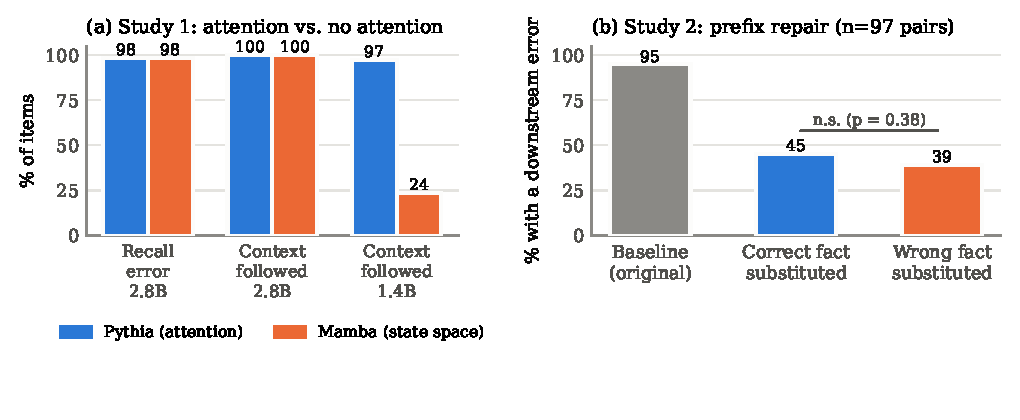
\includegraphics[width=\linewidth]{figures/fig_results.pdf}
\caption{(a) Study~1. At 2.8B, removing attention changes neither free-recall failure (197/200 non-correct for both models) nor adoption of a planted false statement (72/72 for both). At 1.4B the state-space model adopts the planted statement far less often (17/72 vs.\ 70/72). (b) Study~2, on the 97 items where neither substitution was refused. Replacing the first wrong fact roughly halves the share of answers with a downstream error. A different wrong fact does as well as the correct one (exact McNemar $p=0.38$).}
\label{fig:results}
\end{figure}

\begin{table}[t]
\caption{Study 1 results. Each Pythia/Mamba pair shares corpus, tokenizer and approximate parameter count. Probe 1a was run on the 2.8B pair only.}
\label{tab:s1}
\begin{center}
\begin{tabular}{lcccc}
\toprule
Probe and outcome & Pythia-2.8B & Mamba-2.8B & Pythia-1.4B & Mamba-1.4B \\
\midrule
1a correct & 3/200 & 3/200 & -- & -- \\
1a factual error & 187/200 & 195/200 & -- & -- \\
1a abstention & 7/200 & 0/200 & -- & -- \\
1a degenerate & 3/200 & 2/200 & -- & -- \\
\midrule
1b prior correct, no context & 20/24 & 22/24 & 20/24 & 24/24 \\
1b context followed & 72/72 & 72/72 & 70/72 & 17/72 \\
1b prior fallback & 0/72 & 0/72 & 1/72 & 51/72 \\
1b followed: early / middle / late & 24 / 24 / 24 & 24 / 24 / 24 & 23 / 23 / 24 & 7 / 3 / 7 \\
\bottomrule
\end{tabular}
\end{center}
\end{table}

\paragraph{Free recall.} Each model answered 3 of 200 questions correctly (Table~\ref{tab:s1}). Both produced a factual error on 182 of the same questions. Pythia abstained or degenerated on 10 items and Mamba on 2, which accounts for most of the difference in factual-error counts (exact McNemar on the factual-error indicator, $p=0.096$). Both models are near floor, so this probe shows that removing attention does not change recall failure at this scale. It cannot rule out a smaller role for attention in recall.

\paragraph{Context conflict.} At 2.8B both models followed the planted statement on all 72 context items, at every position, so the paired comparison has no discordant pairs. Both models knew most of these facts without context (20/24 and 22/24). At 1.4B the pair separates. Pythia-1.4B followed the planted statement on 70 items. Mamba-1.4B followed it on 17 and gave its prior answer on 51, although it answered all 24 facts correctly without context. All 53 discordant pairs are items Pythia-1.4B followed and Mamba-1.4B did not (exact McNemar $p<10^{-15}$). Qwen2.5-1.5B followed the planted statement on 72 of 72 items. Across the five models, following rates do not differ between the attention group (three models) and the non-attention group (two models; Mann--Whitney $p=0.75$).

\subsection{Interpretation and limits}
\label{sec:s1-limits}

At the matched 2.8B scale, P5 fails on the criterion stated in Section~\ref{sec:framework}: removing attention changed neither free-recall failure nor context adoption. A state-space model of this size adopts a planted false statement as readily as a transformer, so attention is not required for this kind of context-induced error. The 1.4B result would, taken alone, have supported the opposite conclusion. Its disappearance at 2.8B is more consistent with the known weakness of small state-space models at recall from context \citep{arora2024zoology,jelassi2024repeat} than with a mechanism specific to attention. On this reading, Mamba-1.4B gave its prior answer because it did not retrieve the planted line, not because it resisted it.

Three limits apply. (1) Probe~1b is easy: the facts are well known, the texts are short, and both 2.8B models are at ceiling. A harder probe with longer texts, less familiar facts or graded conflict could reveal differences that a ceiling hides. (2) There are two matched pairs and one reference model, so the scale trend rests on two points. (3) Probe~1a is near floor and constrains the recall side only weakly.

%=================================================================
\section{Study 2: Repairing the First Error, With Controls}
\label{sec:study2}
%=================================================================

\subsection{Setup}

\paragraph{Items and models.} We drew a simple random sample of 200 SimpleQA questions with a fixed seed (20260819). Three instruction-tuned models served through the Groq API answered every question at temperature 0, with the system prompt ``Answer the question directly and completely'': GPT-OSS-120B, Qwen3.6-27B (which produces a reasoning trace before answering) and ALLaM-2-7B. Of the 600 responses, 128 stated a wrong fact and followed it with at least one claim building on it. We removed 17 in which the model hedged or refused instead of committing to a single wrong fact (15 from ALLaM-2-7B, 2 from GPT-OSS-120B). The remaining 111 items comprise 72 from ALLaM-2-7B, 21 from Qwen3.6-27B and 18 from GPT-OSS-120B. For each item we recorded the character offset of the first divergence from a correct answer. We wrote two replacements for the divergent span: the SimpleQA gold answer, and a plausible wrong alternative that differs from the model's own error.

\paragraph{Conditions.}
\textbf{A (baseline)}: the original response.
\textbf{B (correct substitution)}: the response up to the divergence, followed by the gold answer, is supplied as a partial assistant turn, and the model continues from it.
\textbf{D (wrong substitution)}: as B, with the alternative wrong fact.
\textbf{C (isolated)}: the question asked again with no prior answer, using the fixed template ``In one clear sentence, what is the correct answer to this: [question]''.

\paragraph{Scoring.} For A, B and D, two annotators counted the claims after the divergence point that the reference contradicts or does not support, and flagged abstentions. For C they scored whether the answer was correct. Both annotators scored all 444 rows independently and blind to condition. Agreement on the presence of any downstream error was $\kappa=0.94$ ($n=333$; exact agreement on the count, 91.6\%). Agreement on isolated correctness ($n=111$) and on abstention ($n=222$) was $\kappa=1.0$. Our main outcome is whether a response contains at least one downstream error. A refusal under B or D contains no claims, so we treat it as missing, not as error-free.

\paragraph{Hypotheses.} The hypotheses, threshold and tests below were fixed before scoring. H1: B reduces the downstream-error rate relative to A by at least 20 percentage points. H2: on items where B removes all downstream errors, the model answers C correctly. H3: B yields fewer downstream errors than D.

\paragraph{Deviations from the planned protocol.} There are six. (1) The original pool of self-written questions produced 0--1 qualifying errors and was replaced with SimpleQA. (2) Qwen3.6-27B's token limit was raised from 1024 to 2048 because its reasoning traces were being truncated. 47 of its 200 responses still truncated and were excluded. (3) The isolated query was reworded with the fixed template above, because at temperature 0 the baseline wording reproduces the baseline answer. (4) The planned test for H3 was a two-proportion $z$-test. B and D are measured on the same items, so we report the exact McNemar test as primary and the planned test next to it. (5) A first analysis indexed items by question only. Seventeen questions produced qualifying errors from two models, so one model's rows overwrote the other's, leaving 90 items. The corrected analysis indexes by question and model and uses all 111. Both scripts are released. (6) The use of one annotator's scores for hypothesis tests, with the other used for reliability, was not specified before scoring. The second annotator's scores lead to the same conclusions (Appendix~\ref{app:s2second}).

\subsection{Results}

\begin{table}[t]
\caption{Study 2 results (primary annotator). A downstream error is at least one failing claim after the divergence point.}
\label{tab:s2}
\begin{center}
\small
\begin{tabular}{@{}lp{4.4cm}cp{4.6cm}@{}}
\toprule
 & Comparison & Result & Test \\
\midrule
H1 & A vs.\ B, share with an error ($n=106$) & 92.5\% $\to$ 48.1\% & exact McNemar, 50 vs.\ 3 discordant, $p=5.5\times10^{-12}$ \\
 & A vs.\ B, failing claims per answer & 1.70 $\to$ 0.75 & Wilcoxon signed-rank, $p=1.8\times10^{-11}$ \\
H2 & C correct where B succeeded ($n=50$) & 1/50 (2.0\%) & Wilson 95\% CI [0.4\%, 10.5\%] \\
H3 & B vs.\ D, share error-free ($n=97$) & 54.6\% vs.\ 60.8\% & exact McNemar, 13 vs.\ 19 discordant, $p=0.38$; planned $z$-test, $z=-0.87$, $p=0.38$ \\
 & B vs.\ D, failing claims per answer & 0.66 vs.\ 0.76 & Wilcoxon signed-rank, $p=0.91$ \\
\midrule
 & C correct, all items ($n=111$) & 2/111 (1.8\%) & -- \\
 & Self-correction within A ($n=111$) & 0/111 & -- \\
 & Refusals under B / D ($n=111$) & 5 / 12 & exact McNemar, 2 vs.\ 9 discordant, $p=0.065$ \\
\bottomrule
\end{tabular}
\end{center}
\end{table}

\paragraph{H1 holds.} With the correct fact inserted, the share of answers containing a downstream error fell from 92.5\% to 48.1\%, a 44.3-point drop against the planned threshold of 20 points (Table~\ref{tab:s2}; Benjamini--Hochberg $q=1.1\times10^{-11}$). The mean number of failing claims per answer fell from 1.70 to 0.75. The direction is the same for each model: ALLaM-2-7B from 94.2\% to 50.7\% ($n=69$, $p=1.5\times10^{-8}$), Qwen3.6-27B from 100\% to 42.1\% ($n=19$, $p=0.001$), GPT-OSS-120B from 77.8\% to 44.4\% ($n=18$, $p=0.11$). No baseline answer corrected itself.

\paragraph{H2 and H3 do not hold.} Asked directly, the models gave the correct answer on 2 of 111 items, both from ALLaM-2-7B. Among the 50 items where the correct fact removed every downstream error, the model knew the answer in isolation for 1. Inserting a different wrong fact reduced downstream errors about as much as inserting the correct one. On the binary outcome the wrong fact did slightly better (60.8\% vs.\ 54.6\% error-free); on the claim count the correct fact did slightly better (0.66 vs.\ 0.76 failing claims). Neither difference is significant. Refusals were more frequent after a wrong substitution (12) than after a correct one (5), a difference that does not reach significance ($p=0.065$).

\paragraph{Length.} Fewer errors could simply reflect shorter continuations. Measured from the divergence point, the median continuation is 29 words in A, 28 in B and 29 in D, so length does not explain the effect.

\subsection{Interpretation}

H1 confirms that what follows depends on what was committed: change the committed fact and about half of the downstream errors disappear. H2 and H3 rule out the stronger explanation on these items. The models did not know the facts, and whether the inserted fact was true made no detectable difference. \citet{zhang2024snowball} built their items from facts the models know, and knowledge-based commitment may operate there. Our items are long-tail SimpleQA questions, where the objective-and-frequency account already predicts failure \citep{kandpal2023}, and the knowledge route is not available. Two explanations remain and the design does not separate them. Any substitution may break a chain of elaboration that the original fact supported. Alternatively, some downstream claims in the baseline may be independent fabrications that a new prefix happens to produce less often, regardless of what the prefix says. The T1 attribution rule requires both a successful repair and correct isolated knowledge; it assigns 1 of 111 errors to commitment.

%=================================================================
\section{Discussion}
\label{sec:discussion}
%=================================================================

\paragraph{What the studies support.} Neither of the two mechanistic attributions we tested survived its control. Attention was not required for context-induced errors at the matched 2.8B scale, and the commitment effect did not depend on the model knowing the correct answer. Both effects are real as behaviour: models adopt planted statements, and downstream claims depend on what was committed. What failed is the assignment of each behaviour to the component that the framework predicted. For the long-tail errors in Study~2, the most likely source is the objective-and-frequency component, since the models did not have the facts. Our companion study, a separate pre-registered evaluation of five open-weight models (5{,}620 dual-scored responses; anonymised data, code and pre-registration in the supplementary material), found error rates of 65.5\% on niche-domain questions against 43.3\% on general-domain questions (odds ratio 2.49), and 77.4\% of incorrect answers carried no hedge. This is consistent with that reading, although it measures error rates and does not attribute individual errors.

\paragraph{A component label alongside the output label.} The results support recording, for each error, both its output type and the component an intervention attributes it to. Consider two extrinsic errors. One disappears when a misleading passage is removed; the other persists under a minimal prompt. The first calls for context filtering, the second for adding knowledge or abstaining, yet both receive the same output label. Both studies show that the component label has to come from a controlled intervention. In Study~1, the 1.4B pair alone would have attributed context adoption to attention; the 2.8B pair shows that attribution would have been wrong. In Study~2, the repair that worked would have been attributed to commitment, and the wrong-fact control shows that attribution would have been wrong too.

\paragraph{Practical consequences.} For retrieval-augmented systems, Study~1 shows that four of five models adopted a planted false statement on at least 70 of 72 items, with and without attention, so the choice of sequence mixer is not a defence against misleading context; filtering what enters the context is. For decoding-time correction, Study~2 indicates that rewriting an early claim reduces later errors even when the rewrite is wrong. A pipeline that reports fewer errors after self-revision has therefore not shown that its content is more accurate.

%=================================================================
\section{Limitations}
\label{sec:limits}
%=================================================================

Study~1 uses two matched pairs, at 1.4B and 2.8B parameters, and a context probe on which the 2.8B models are at ceiling. Study~2 uses long-tail questions on which the models almost never know the answer. That choice produced enough errors to analyse, but it is the setting least favourable to knowledge-based commitment. The direct follow-up is an item set restricted to questions each model answers correctly in isolation. ALLaM-2-7B supplies 72 of 111 items, so per-model estimates for the other two models are imprecise. Of the three interventions, only T1 and the architecture substitution were run; the position test (T2), the frequency test (T3) and a classifier baseline for attribution labels are left for future work. The annotators are also authors. Blind scoring and high agreement reduce the risk of expectation effects but do not remove it.

%=================================================================
\section{Conclusion}
\label{sec:conclusion}
%=================================================================

Output taxonomies identify the type of an error but not its source. Interventions that need only sampling access can test hypotheses about the source. In Pythia and Mamba models matched on data and scale, removing attention at 2.8B left both free-recall failure and adoption of misleading context unchanged; a difference at 1.4B disappeared at the larger scale. In three instruction-tuned models, replacing the first error in a long-tail answer halved the errors that followed, whether or not the replacement was true, and the models rarely knew the correct answer. In both cases the plausible mechanistic reading of a strong effect failed a control. Component attribution needs comparisons across scale and matched counterfactual inputs before a label is assigned.

\subsubsection*{Broader Impact Statement}
The work aims to make confident model errors easier to diagnose. It uses public benchmarks and publicly available models and involves no personal data. Probe 1b confirms that models readily adopt false statements placed in their context. This is already well documented, and we release no tooling for producing such inputs beyond the probe items themselves.

\subsubsection*{Reproducibility Statement}
The supplementary material contains, for both studies, the raw model outputs, blind scoring sheets, model key, both annotators' files and the analysis scripts, including the original and corrected Study~2 analyses, together with the anonymised companion-study materials cited in Section~\ref{sec:discussion}. Each folder's README lists the commands that reproduce the reported numbers. Study~1 runs on a single 8\,GB GPU. Both question samples can be regenerated from fixed seeds. The Study~2 protocol and all deviations from it are described in Section~\ref{sec:study2}.

\bibliography{references}
\bibliographystyle{tmlr}

\appendix

\section{Study 2: Second Annotator}
\label{app:s2second}
With the second annotator's scores and the same corrected analysis: H1, 97.2\% $\to$ 50.0\% ($n=106$; 51 vs.\ 1 discordant; $p=2.4\times10^{-14}$); H2, 1 of 51 correct in isolation; H3, 52.6\% vs.\ 57.7\% error-free ($n=97$; 13 vs.\ 18 discordant; $p=0.47$).

\section{Study 2: Example Item}
Question: ``Who developed Japan's first arc lamp?'' (gold answer: Ichisuke Fujioka). GPT-OSS-120B names a different engineer and then adds an employer and a demonstration city. Condition B replaces the name with ``Ichisuke Fujioka''; condition D replaces it with ``Shoichi Tanaka'', which is plausible but wrong. In both, the model continues from the inserted name.

\end{document}
